\documentclass[12pt]{article}
\usepackage{amsmath}
\usepackage{parskip}
\usepackage{graphicx}
\usepackage[letterpaper, margin=1in]{geometry}
\usepackage{fancyhdr}
\fancypagestyle{prelabheader} {
    \rhead{Raeed Hassan \\ hassam41}
    \lhead{\huge{ELECENG 2CI5 Lab 6 Prelab}}
}
\graphicspath{{./images/}}

\begin{document}
\newgeometry{margin=1in, includehead, head=47pt}
\thispagestyle{prelabheader}
i. \\
The measured value of the Thevenin voltage, $V_{TH}$, is equal the voltage measured across $V_o$ after creating an open circuit, and is measured to be $3.142V$. The Thevenin resistance, $R_{TH}$, is calculated from creating a short circuit across the voltage source and then finding the equivalent resistance across the circuit (excluding $R_o$). $R_{TH} = (R1||R2||R4||R5) = 174.05\Omega$. \\
\begin{center}
    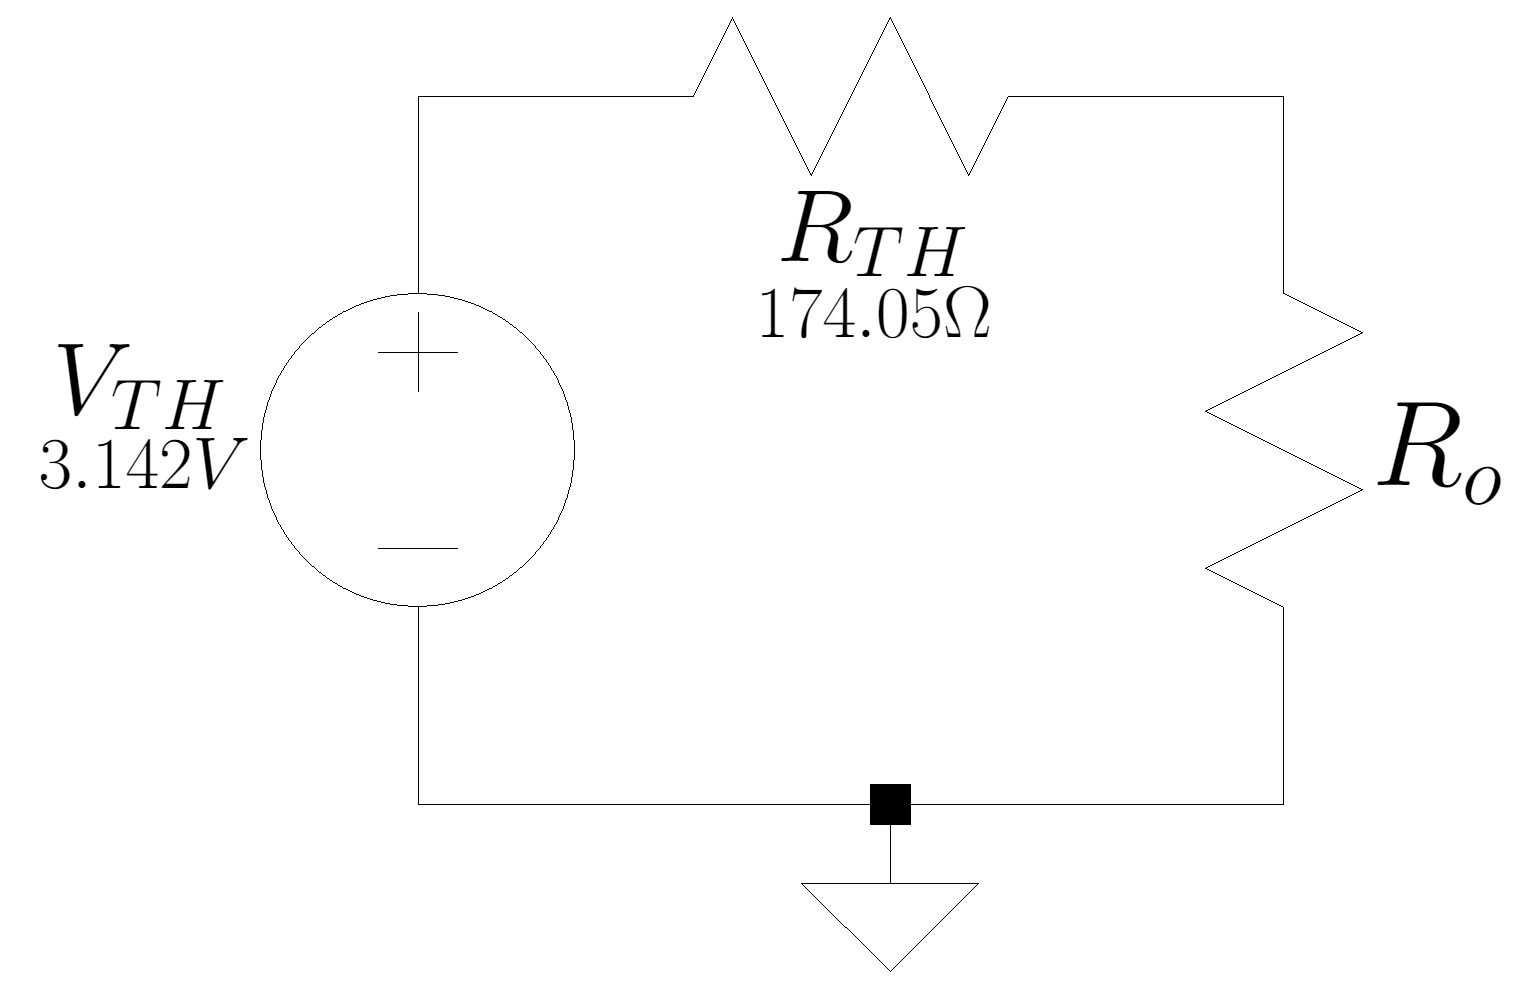
\includegraphics[width=0.6\textwidth]{thevenincircuit.png}
\end{center}

ii. \\
The value of $I_N$ is equal to the value of the $I_{SC}$ when the Thevenin equivalent circuit is short circuited at the load, therefore $I_N = I_{SC} = \frac{V_{TH}}{R_{TH}} = \frac{3.142V}{174.05\Omega} = 18.05mA$. The Norton resistance, $R_N$, is equal to the Thevenin resistance of the Thevenin equivalent circuit, therefore $R_N = R_{TH} = 174.05\Omega$. \\
\begin{center}
    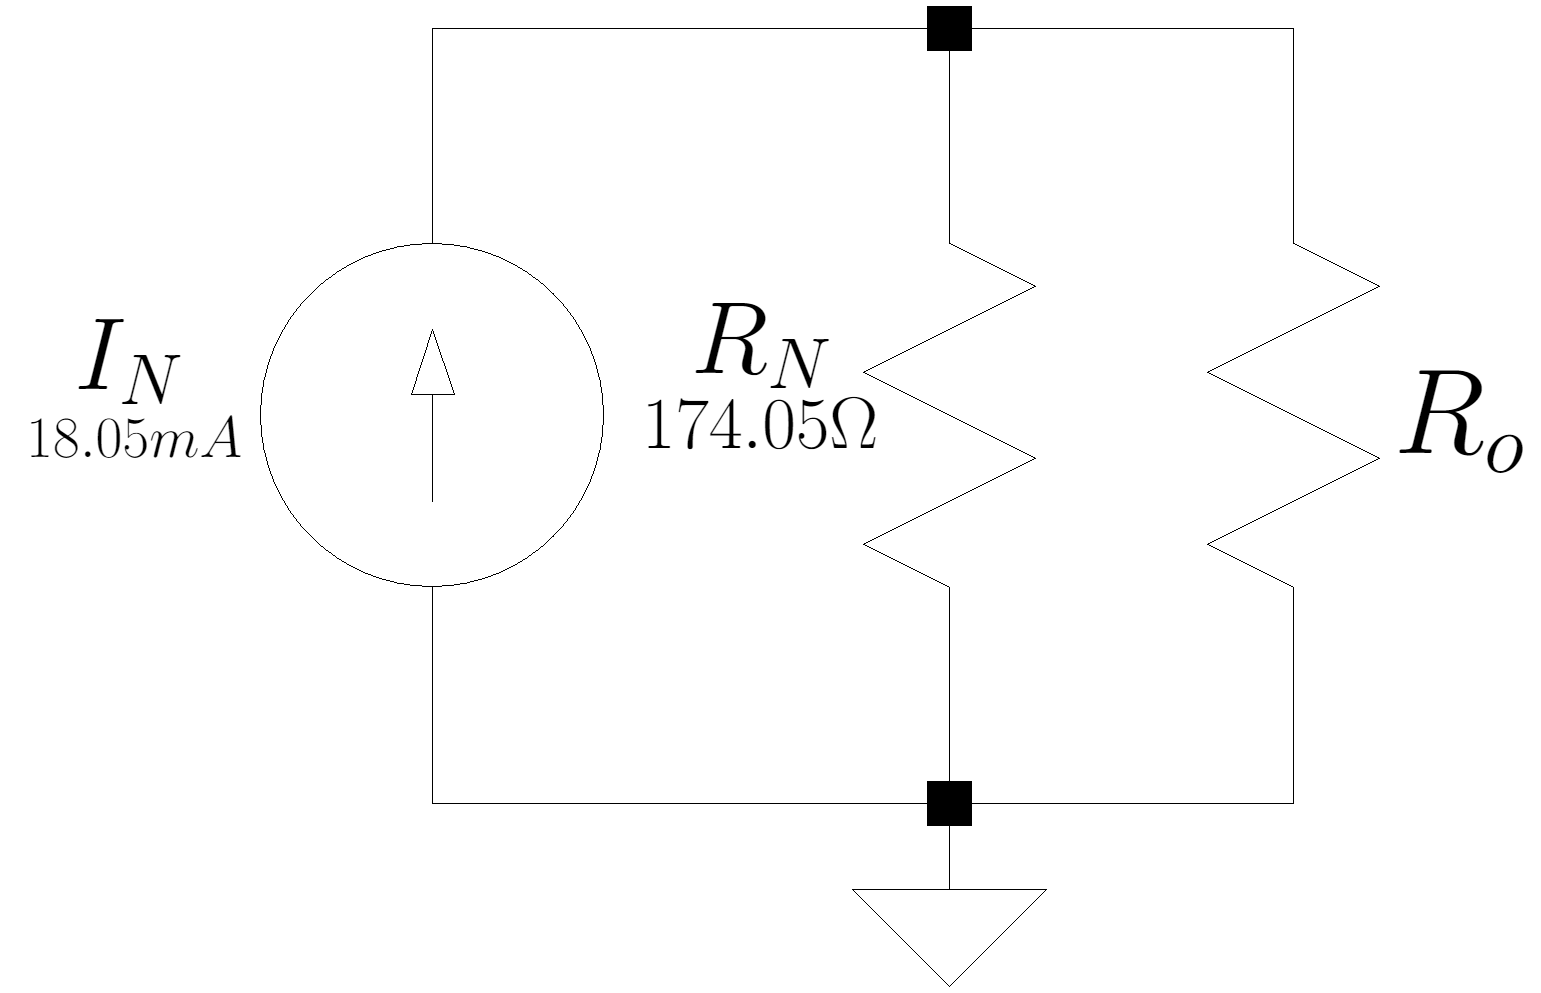
\includegraphics[width=0.6\textwidth]{nortoncircuit.png}
\end{center}
\restoregeometry
\clearpage
iii. \\ The value of $R_o$ that would allow for the maximum power transfer in this circuit is $174.05\Omega$. This is because the derivative of the power in a Thevenin/Norton circuit is equal to zero when the load resistance is equal to the Thevenin/Norton resistance.

iv. \\ 
\[P_{max} = I^2R_o = (\frac{V}{R_o+R_{TH}})^2R_o = (\frac{3.142}{174.05+174.05})^{2}174.05 = 14.18 mW\] \\ 
The maximum power transfer in the circuit is $14.18 mW$.

v. \\ The theoretical value for $R_{TH}$ can be calculated by creating a short circuit around the voltage source and then finding the equivalent resistance of the circuit (excluding the load resistor, $R_o$). $R_{TH} = (R1\,||\,R2\,||\,R4\,||\,R5) = (220\,||\,1k\,||\,10k\,||\,10k) = 174.05\Omega$. The theoretical value for $V_{TH}$ can be found by creating an open circuit around $V_o$ and calculating the open circuit voltage. We can use nodal analysis, there is a single node with voltage at that node equal to the open circuit voltage, $V_{oc}$.
\[
\begin{bmatrix}
    \frac{1}{220} + \frac{1}{1k} + \frac{1}{10k} + \frac{1}{10k}
\end{bmatrix}
\begin{bmatrix}
    V_1
\end{bmatrix}
=
\begin{bmatrix}
    \frac{4V}{220}
\end{bmatrix}
\]
\[
\begin{bmatrix}
    V_1
\end{bmatrix}
=
\begin{bmatrix}
    \frac{1}{220} + \frac{1}{1k} + \frac{1}{10k} + \frac{1}{10k}
\end{bmatrix}^{-1}
\begin{bmatrix}
    \frac{4V}{220}
\end{bmatrix} 
\]
\[
\begin{bmatrix}
    V_1
\end{bmatrix}
=
\begin{bmatrix}
    3.1642V
\end{bmatrix}
\]
After performing nodal analysis, we can see that $V_{TH} = V_1 = 3.1642V$. The measured value of $V_{TH}$, $3.142V$, is very similar to the calculated value of $V_{TH}$, $3.1642V$.

vi. \\ The resistor used had a resistance of $220\Omega$. The voltage for the Thevenin circuit using a similar resistance to the Thevenin resistance is similar to the voltage of the original circuit.
\begin{center}
    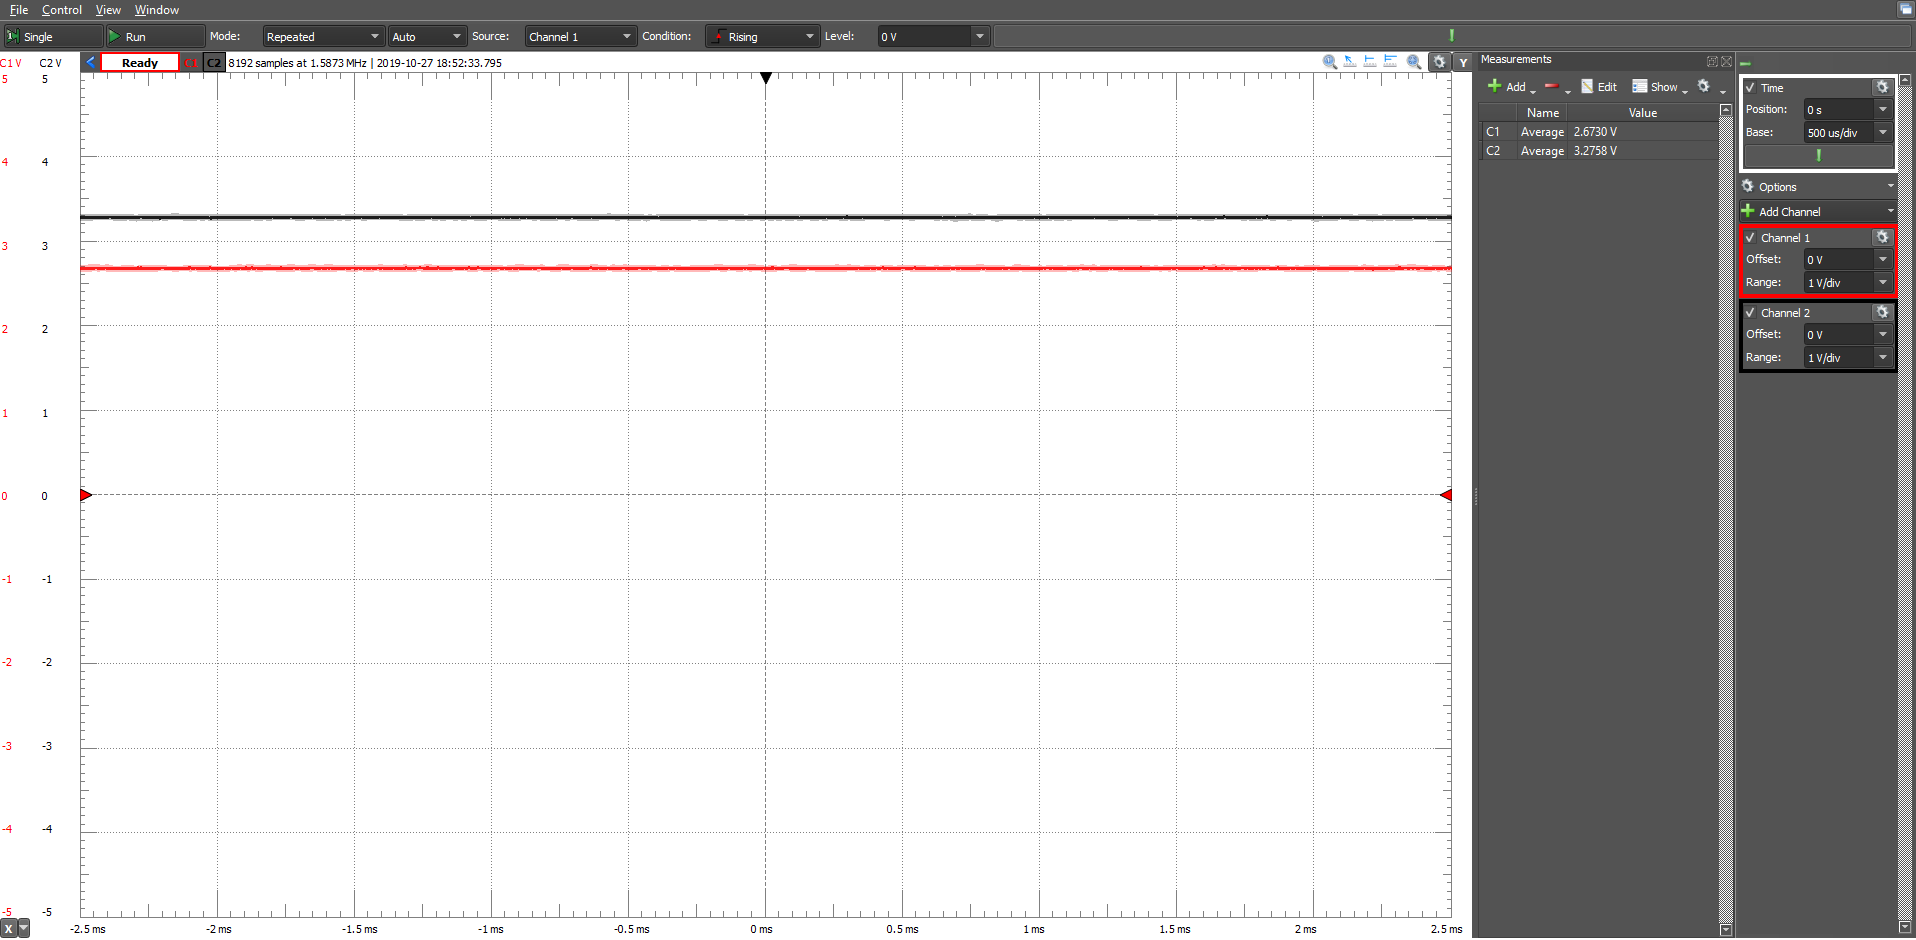
\includegraphics[width=0.93\textwidth]{prelab6part6.png}
\end{center}

\end{document}